% \section{Problem Definition}

\section{Dynamic Multi-Domain Problem}
\label{appdix:task}
We clarify the $\mathbf{DMPC}$ problem as follows. Given a set $\mathcal{G}$ of $n$ relatively independent label taxonomies at initial time $t_0$
$$
\{G_1, G_2, G_3, ..., G_n\},
$$
each of which correlates with a domain-specific product categorization task. The taxonomy of product categories $G_i$ is tree-structured with depth $d_i$, and it contains $m_i$ category leaf nodes:
$$
\{y_i^{(1)}, y_i^{(2)}, y_i^{(3)}, ..., y_i^{(m_i)}\} \subseteq G_i.
$$
% As time $t_{>0}$ goes, the category node $y_i^{(a)}$ might be \textbf{divided} into two categories $y_i^{(a1)}$ and $y_i^{(a2)}$ or be  \textbf{integrated} with another category $y_i^{(b)}$ to form $y_i^{(ab)}$. The \textbf{new} category node $y_i^{(m+1)}$ with corresponding products can also appear and the extreme scenario is that an emerging taxonomy $G_{n+1}$ sprouts along with the new business development from another domain.
Part of the nodes is enrolling in a dynamic trending. As time goes $t_{>0}$, the category node $y_i^{(a)}$ of a certain product might be \textbf{divided} into two categories $y_i^{(a1)}$ and $y_i^{(a2)}$ or \textbf{integrated} with another category $y_i^{(b)}$ to form $y_i^{(ab)}$. The \textbf{emergence} of a new category node $y_i^{(m+1)}$ with corresponding product titles is also possible.
In addition, an emerging taxonomy $G_{n+1}$ may sprout when a new business is cultivated.

\cut{
A qualified system is supposed to
\begin{enumerate}
    \item jointly handle the $n$ static product taxonomy classification tasks at time $t_0$;
    \item sustain classification accuracy when the above taxonomy evolving issues are encountered;
    \item resume tolerable performance when zero-shot transfer to new taxonomy to improve cold-start user experience.
\end{enumerate}
}

% \subsection{Task Reformulation}
A single product categorization task on taxonomy $G_i$ ($i=1$) is a traditional classification task, in which the training data and test data are organized in tuples 
$$
\mathcal{S}=\{(X_i^{(1)}, y_i^{(1)}),...,(X_i^{(m_i)}, y_i^{(m_i)}),...\}.
$$
Each $X_i$ in $\mathcal{S}$ represents the title of one product and $y_i$ is the corresponding class node in the categorical taxonomy tree.

In $\mathbf{DMPC}$ problem, when $i \geq 2$, to unify the training data and the inference procedure cross $G_i$, 
% we aim to match $X_i$ and $y_i$. 
we reformulate classification as the matching between $X_i$ and $y_i$. 
While traditional classifiers regard $y_i$ as meaningless label ordinals, we instead treat them along the path of top-bottom taxonomy nodes equivalently with the product title as free text. 
In this reformulated text semantic similarity matching task, the data samples are:
\begin{equation*}
\begin{split}
        \mathcal{S}_i=\{&(X_i^{(1)}, y_i^{(1)}, Y_{\mathbbm{1}}^{(1)}),...,\\
        &(X_i^{(m_i)}, y_i^{(m_i)}, Y_{\mathbbm{1}}^{(m_i)}),...\},
\end{split}
\end{equation*}
$$
\mathcal{S}=\{\mathcal{S}_1, \mathcal{S}_2,...,\mathcal{S}_i\},
$$
where $Y_{\mathbbm{1}}\in \{0, 1\}$ is an indicator denoting whether the text pair $X_i$ and $y_i$ is matched ($Y_{\mathbbm{1}}=1$) or not ($Y_{\mathbbm{1}}=0$).

% This reformulation is especially advantageous to simultaneously (i) capture the semantic relatedness of product titles and label texts and (ii) handle multiple taxonomies \& taxonomy evolving issues in a zero-shot manner without re-training once a unified system is well established.
% ,considering that the label text already contains rich information of this category.

\section{Details of Meta Concept Set Construction and Tagging}
\label{sec:datasetdetails}
Meta concepts are fine-grained tags that have been widely used in industrial knowledge graphs (e.g. Amazon~\cite{dong2020autoknow}, Walmart~\cite{xu2020product}, Alibaba~\cite{luo2020alicoco}). 
Details of meta concept construction and tagging are listed below. We will use ``concept" instead of ``meta concept'' for brevity.
% The construction includes concept mining, concept recall and concept classification.

\subsection{Concept Set Construction}

% Concept mining. 
Concept set construction is conducted in a semi-supervised manner.
First, we use a domain-specific named entity recognition (NER) model to mine fine-grained entities from product titles. These entities are complemented with queries from search engine and cumulated knowledge from experts to form the initial pool of concepts. 
Based on that, we use a naive classifier to pick-up high-quality concepts with high search frequency or broad product coverage. 
Then, manual annotation is performed on the remaining 20k entities, achieving 95\% accuracy in quality checking.
Finally, we collect over 30k concepts covering the most fine-grained knowledge in product titles.

\subsection{Concept Tagging}
Concept tagging is comprised of two stages.

The first stage is concept recall. 
In order to find candidate concepts for each product, we adopt three approaches: NER, knowledge reduction and semantic recall. 
First, seed candidates are found by NER on product titles.
% which is the same as the procedure in concept mining. 
Second, we extend seed candidates with their neighbors in commonsense knowledge graphs, such as synonyms and brand-concept relations (some brands sell specific products). 
Third, for those products without seed candidates, we use Sentence-BERT to retrieve concepts by textual semantics.
The low-quality concepts recalled will be filtered in the next stage, i.e. concept classification. 
% However, the recall model is trained on similar dataset to the concept classification model, which results in few low-quality concepts have passed the filtering. To overcome this problem, we turn to use the knowledge in domain specific pretraining, especially the mask language model (MLM) task. Concretely, we recognized named-entities in product title and insert [MASK] into these entities to form a new title. Then we try to generate entity at the [MASK] from the new title, which is the same as MLM in pretraining. 
% With this method, we achieve 50\% increment on uncoverage products with high precision.

The second stage is concept classification. Based on the candidates collected in the previos stage, we train a binary classifier to filter out concepts which attain low relevance score with product titles. The classifier is fine-tuned with knowledge integration which will be introduced in our successive work.

% \begin{figure}[tbp]
%   \centering
%   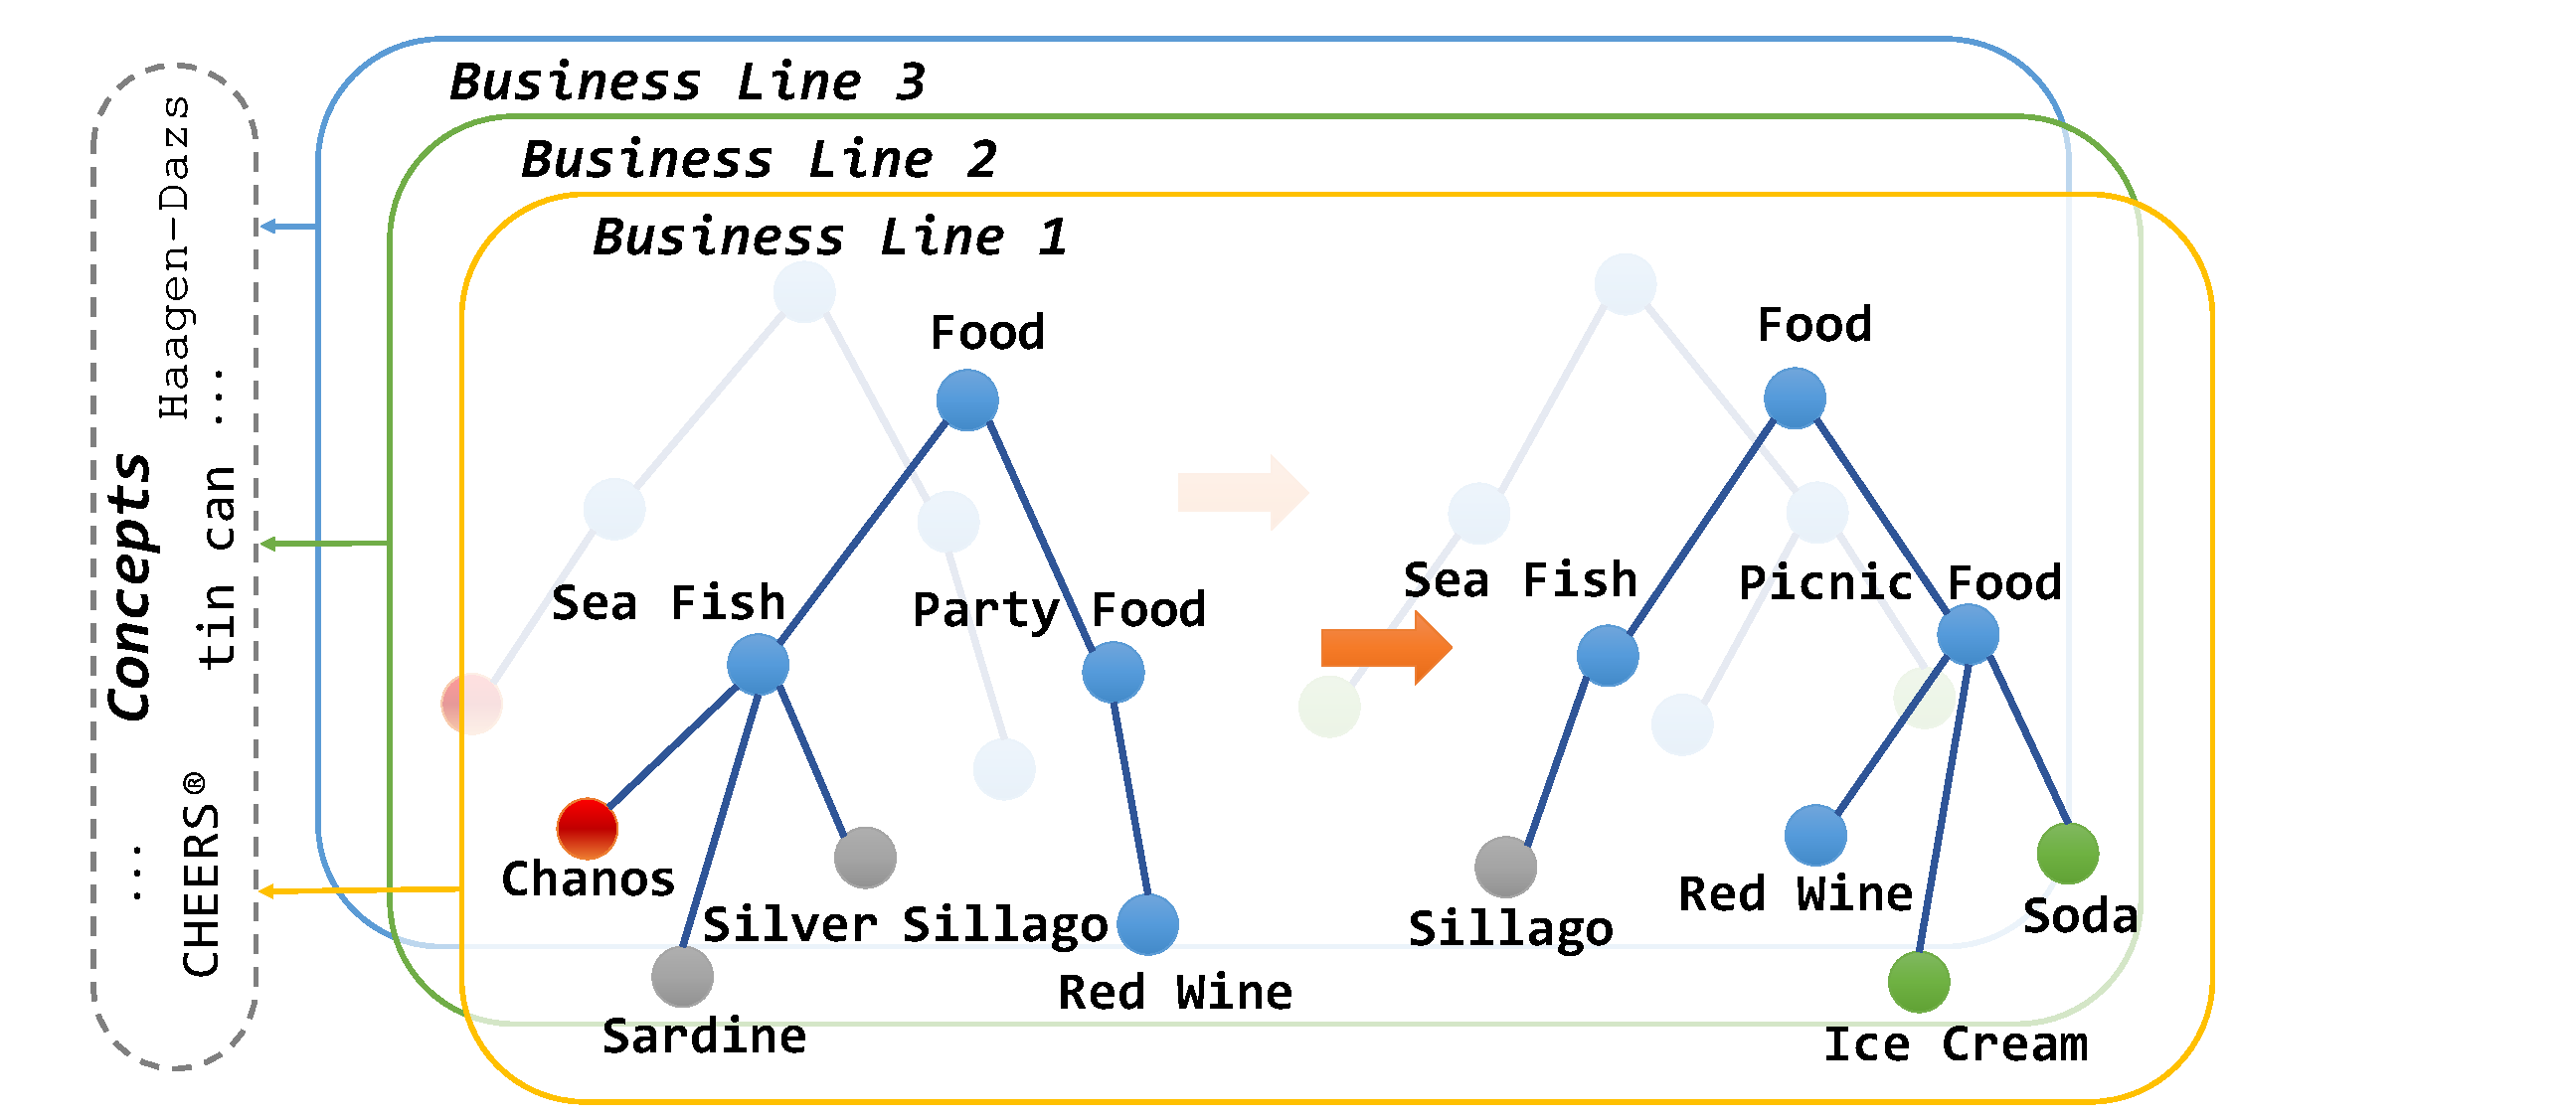
\includegraphics[width=\linewidth]{fig1}
%   \caption{
% %   An illustration of multiple taxonomies and taxonomy evolving. 
%   Multiple taxonomies from different business lines are evolving themselves, including node deletion, integration, increment, and so on. But the fine-grained concepts of products seldom shift. }
%   \label{fig:teaser}
% \end{figure}
\section{Implementation Details}
% \paragraph{Implementation Details}
\label{appdix:exp detail}
For fair comparisons, 
% We deploy all experiments on Nvidia Geforce A100 80G GPU.
all the ``BERT'' abbreviations mentioned in this work are Google BERT-base pretrained on Chinese corpus. 
For TF-IDF and FastText baselines, We use jieba
\footnote{\href{https://github.com/fxsjy/jieba}{https://github.com/fxsjy/jieba}}
toolkit to generate Chinese word segments and tune hyper-parameters on each dataset respectively. 
BERT-related models are initialized from the pretrained Google BERT-base (Chinese) and tuned with 2e-5 learning rate, 512 batch size, 32 sequence length, except that the cross-encoder BERT in \textit{Reranking} stage extends the sequence length to 64. 
All BERT related appoaches are trained 40 epochs while multi-task baseline trained at most 120 epochs. 

% \TODO{resize table}
\begin{table}[th]
    \small
  % \setlength{\tabcolsep}{2.5pt}
  \caption{Examples from the three Datasets}
  \label{tb:exa}
  \centering
  \begin{tabular}{c|c}
    \toprule
     Product title  & Taxonomy path \\
     \midrule
     \multicolumn{2}{c}{QD}\\
     \midrule
      \tabincell{c}{\textit{Towel gourd 1 pcs} \\ \textit{\& soy bean 150g}} & \tabincell{c}{\small{Vegetable} $\rightarrow$ \small{Mixed Product} \\ $\rightarrow$  \small{Vegetables mixture}} \\
    %  \midrule
     \multicolumn{2}{l}{\tabincell{l}{\\Concepts:\{$\left\langle \mathtt{soy\;bean}\right\rangle$, $\left\langle \mathtt{towel\;gourd}\right\rangle$\}}}\\
     \midrule
     \multicolumn{2}{c}{BH}\\
     \midrule
     \tabincell{c}{\textit{Fresh bamboo shoots} \\ \textit{(dig from mountains)}} & \tabincell{c}{\small{Vegetable/Fruit} $\rightarrow$ \small{Vegetable} \\$\rightarrow$ \small{Tubers} $\rightarrow$ \small{Bamboo}} \\
    %  \midrule
     \multicolumn{2}{l}{\tabincell{l}{\\Concepts:\{$\left\langle \mathtt{bamboo\;shoot}\right\rangle$, $\left\langle \mathtt{native\;product}\right\rangle$\}}}\\
     \midrule
     \multicolumn{2}{c}{FG}\\
     \midrule
     \tabincell{c}{\textit{Butter leaf lettuce 100g}} & \tabincell{c}{\small{Fresh} $\rightarrow$ \small{Vegetable} $\rightarrow$ \\ \small{Leaf} $\rightarrow$ \small{Lettuce}}\\
    %  \midrule
     \multicolumn{2}{l}{\tabincell{l}{\\Concepts:\{$\left\langle \mathtt{lettuce}\right\rangle$, $\left\langle \mathtt{butter\;lettuce}\right\rangle$\}}}\\
     
    \bottomrule
  \end{tabular}
\end{table}

\section{Experiment Analysis}
\subsection{Details of Dense Scorer}
\label{sec:appendix-dense}
In \textit{Retrieval} stage, it is encouraged to exploit the potential candidates as accurately as possible, otherwise the latter \textit{Reranking} stage would never make right predictions if the true label is not covered by the retrieved candidates. Hence we use HR@$k$ to measure the retrieval performance.

We compare several alternatives of the loss function for Dense Scorer, specifically, different approaches for $(\mathbf{u}_x, \mathbf{v}_y)$ similarity measurement. The loss used in \eqnref{eq:loss} is termed as Cosent loss\footnote{This name is after \href{https://kexue.fm/archives/8847}{https://kexue.fm/archives/8847}}. Besides this, one straightforward method is to compute the cosine similarity between vector $\mathbf{u}_x$ and $\mathbf{v}_y$ and optimize the model using vanilla binary cross entropy loss.
\begin{equation}
    \delta=\textit{cos}(\mathbf{u}_x,\mathbf{v}_y)=\frac{<\mathbf{u}_x, \mathbf{v}_y>}{||\mathbf{u}_x||\,||\mathbf{v}_y||},
\end{equation}
\begin{equation}
\label{eq:bce}
    \mathcal{L}^{bce}=-\sum_{S} Y_{\mathbbm{1}} \log(\delta) + (1-Y_{\mathbbm{1}})\log(1-\delta),
\end{equation}
where $Y_{\mathbbm{1}}$ is the binary class.
For the sake of the alignment between embedding $\mathbf{u}_x$ and $\mathbf{v}_y$, we also refer to the classification objective function in SBERT~\cite{reimers2019sentence}.
\begin{equation}
    o=softmax(W_o(\mathbf{u}_x, \mathbf{v}_y, |\mathbf{u}_x-\mathbf{v}_y|)),
\end{equation}
where $W_o\in \mathbb{R}^{3l\times 2}$ is the weighting parameter to project the concatenation of $\mathbf{u}_x$, $\mathbf{v}_y$ and the element-wise difference $|\mathbf{u}_x-\mathbf{v}_y|$ to binary classes. $l$ is the dimension of embeddings. The second element in vector $o$ can be regarded as the probability whether $\mathbf{u}_x$ and $\mathbf{v}_y$ are matched or not, hence we can adopt the same binary cross entropy loss function in \eqnref{eq:bce} to optimize the model.

In \figref{fig:vector-retri}, as $k$ goes on, the HR score increases, and the model trained with Cosent loss is consistently better than others, while the model trained with SBERT loss performs unstably, sometimes worse than Cosine loss. 
One explanation is that comparing with Cosine loss and SBERT loss, the Cosent loss focuses on the positive-versus-negative pairwise optimization, which means the model only cares for the relative order of the prediction results instead of the specific value. And this setting brings consistent recall of candidates.
% \begin{table}[th]
%   \caption{The retrieval results of the vector-based unit over different loss function. The best results are bolded.}
%   \label{tb:vector-retrieval}
%   \centering
%   \begin{tabular}{c|c|ccc}
%     \toprule
%     Loss & Dataset & HR@1 & HR@5 & HR@10 \\
%     \midrule
%     \multirow{3}{*}{Cosine} & QD & 74.80 & 82.28 & 84.46\\
%     & BH & 72.75 & 81.77& 84.04\\
%     & FG & 65.59 & 80.40 & 83.23\\
%     \midrule
%     \multirow{3}{*}{SBERT} & QD & 82.25 & 88.96 & 90.92\\
%     & BH & 76.95 & 86.76 & 89.41\\
%     & FG & 80.67 & 87.27 & 88.86\\
%     \midrule
%     \multirow{3}{*}{Cosent} & QD & 84.19 & 88.97 & 90.30\\
%     & BH & 77.64 & 85.27 & 87.18\\
%     & FG & 82.72 & 86.66 & 87.48\\
%     \bottomrule
%   \end{tabular}
% \end{table}

\begin{figure}
  \begin{subfigure}[b]{0.49\columnwidth}
  \centering
  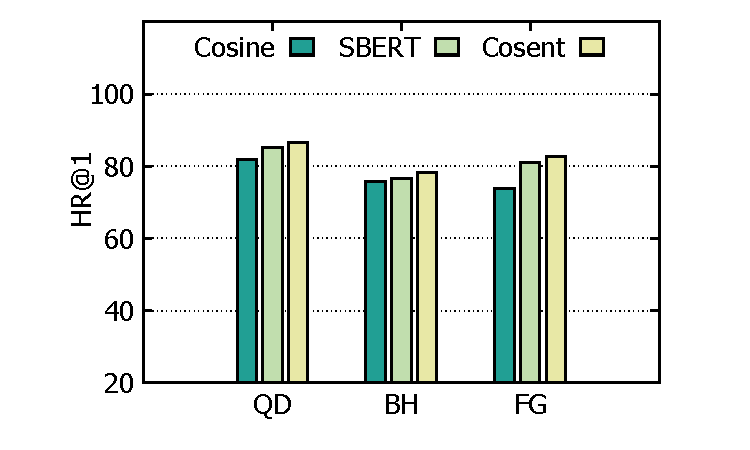
\includegraphics[width=\columnwidth]{hr_1.pdf}
  \caption{HR@1}
  \end{subfigure}
%   \hfill
%   \begin{subfigure}[b]{0.49\columnwidth}
%   \centering
%   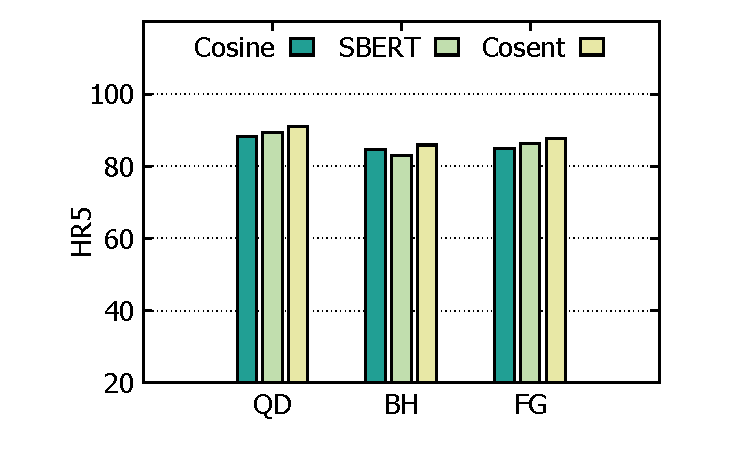
\includegraphics[width=\columnwidth]{hr_5.pdf}
%   \caption{HR@5}
%   \end{subfigure}
  \hfill
  \begin{subfigure}[b]{0.49\columnwidth}
  \centering
  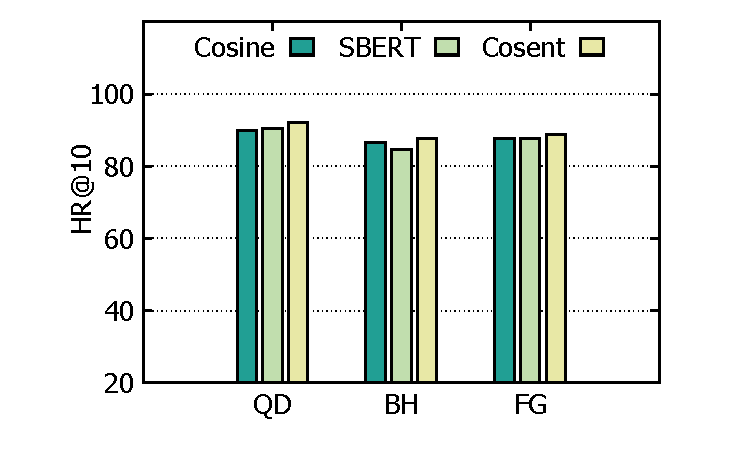
\includegraphics[width=\columnwidth]{hr_10.pdf}
  \caption{HR@10}
  \end{subfigure}
  \caption{The retrieval results of the vector-based unit over different loss functions.}
  \label{fig:vector-retri}
\end{figure}

\subsection{Case Study}
\label{sec:appdix-case}
For product \textit{``New Farmer$^\circledR$ walnut flavored sunflower seed 160g''} which should be categorized into [$\mathtt{Sunflower\,Seed}$], $\mathsf{TaLR}$ without contrastive learning wrongly assign it to [$\mathtt{Walnuts}$]; When concept ``sunflower seed'' is incorporated in contrastive pretraining, $\mathsf{TaLR}$ is capable of distinguishing the right answer.
For product \textit{``CELSIUS$^\circledR$ cola flavored 300ml''} which should belong to [$\mathtt{Sports\,Drink}$], $\mathsf{TaLR}$ without mapping scorer wrongly label it as [$\mathtt{Cola}$]; When concept ``CELSIUS$^\circledR$'' is engaged in retrieval, $\mathsf{TaLR}$ could finally sort out the answer.

\section{Related Work}
\paragraph{Clarification Question Generation} The concept of CQ can be naturally raised in a dialogue system where the speech recognition results tend to be erroneous so that we raise CQs for sanity check \citep{stoyanchev2014towards}, or the intents for a task is incomplete or ambiguous in a first short utterance and further CQs are needed to fill in the slots \citep{dhole2020resolving}. The concept is then extended to IR to clarify ambiguous queries \citep{aliannejadi2019asking}, and has been successfully put into practice \citep{zamani2020generating}. Other application areas including KBQA \citep{xu2019asking} and open-domain dialogue systems \citep{aliannejadi2020convai3}. CQGen can also be applied to help refine posts on websites like StackExchange \citep{Kumar_2020} and Amazon \citep{rao2019answer}. In this context, our work closely follows the research line of \citep{rao2018learning, rao2019answer, cao2019controlling}. \citet{rao2018learning} first adopted a retrieval-then-rank approach. They \citep{rao2019answer} then proposed a generation approach to train the model to maximize the utility of the hypothetical answer for the questions with GAN, to better promote specificity. \citet{cao2019controlling} propose to control the specificity by training on data with explicit indicator of specificity, but it requires additional specificity annotation. Towards the similar specificity goal, we adopted a different keyword-based approach. They also assume generating one question per context, which we claim is not sufficient to cover various possible information needs, and thus propose the task of the diverse CQGen.

\paragraph{Diverse Generation} The demand for diverse generation exists in many other fields~\cite{vijayakumar2018diverse, LiangZ18code, shen2019mixture}, and we've drawn inspirations from these literatures. For image captioning, we may use multiple descriptions for different focusing points of a scene. \textit{Diverse Beam Search} \citep{vijayakumar2018diverse} was proposed to broaden the searching space to catch such diversity by dividing groups in decoding and imposing repetition penalty between them. For machine translation, a context can be translated with different styles. \citet{shen2019mixture} thus proposed \textit{Mixture of Expert} models including hMup to reflect various styles with a discrete latent variable (\textit{expert}). And here for CQGen, diversity is required to cover various potentially missing aspects, so we come up with the idea to use keywords as a controlling variable like \textit{expert} to promote diversity.

